\chapter{SLIM5}
\label{chap:SLIM5}
In this Chapter the SLIM5 R\&D project will be presented. After a short summary of the project 
motivations, goals and timeline (Section~\ref{sec:SLIM5Project}), the Physics motivations of 
and the tracker requirements for SuperB and ILC will be briefly discussed. 
The pixel  (Section~\ref{sec:Apsel4D}) and strip (Section~\ref{sec:Striplets}) 
detector prototypes developed 
within the SLIM5 will be presented. Finally, in Section~\ref{sec:SLIM5Results} the results 
in~\cite{BETTARINI2010942,BOMBEN2010159,NERI2010195} will be discussed.


\section{The SLIM5 Project}
\label{sec:SLIM5Project}
The SLIM5 project~\cite{SLIM5:proj} aimed at advancing the state-of-the-art in the development of thin 
tracking systems to be applied in High-Energy Physics. The project was financed for three years
 (2006-2008) by INFN - National Scientific Committee 5~\cite{INFN_V} and involved several 
 italian research institutes. 
 
 The SLIM5 collaboration worked on developing tracking systems for experiments at 
 high luminosity flavour 
 factories, like the proposed SuperB (\cite{Baszczyk:2013xua}) and linear colliders. The goal was to deliver thin silicon tracking detectors with possibility 
 of self-triggering thanks to the combination of data-driven data acquisition and pattern matching 
 algorithm with very low latency.
Let's know see the required performance for such detectors. 

\section{Tracking and Vertexing Requirements for SuperB and ILC Experiments}
Experiments at high luminosity colliders have to accomplish a high precision measurements 
exploiting at maximum the large dataset they are expected to integrate. 
This means that the experiments have to be very efficient and show excellent performance, 
even in presence of a very intense particle rate; this is particularly true for the tracking and 
vertexing detectors, which are the closest to the beams interaction point. It has also to be stressed 
that with sub-optimal tracking and vertexing performance there's no physics case for such 
experiments; hence the tracking and vertexing detectors are the crucial parts of experiments at 
high luminosity colliders.

We now review quickly some physics cases for SuperB and ILC and the related constraints on 
tracking detectors.
\subsection{SuperB}

The SuperB project~\cite{Baszczyk:2013xua} was the proposal of a super flavour $\epem$ factory operating at the 
 center-of-mass energy of the \Y4S, capable of an instantaneous 
 luminosity of  $10^{36}\cms$, with the goal of integrating 50--75~\invab.

The SuperB physics program was to 
\begin{itemize}
\item[a)]determine the flavor structure of whatever New Physics discovered at the LHC, 
using the information on rare $b$, $c$, and $\tau$ decays, and on \CP
violation in $b$ and $c$ quark decays, or, if  signatures of New Physics were not observed at the LHC,
then
\item[b)]  exploit the excellent sensitivity provided at the luminosity frontier by
a super $B$ factory, to
observing New Physics at mass scales up to 10~\tev or more through
observation of rare processes involving $B$ and $D$ mesons and studies
of lepton flavour violation in $\tau$ decays.
\end{itemize}

The SuperB detector concept was based on the \babar\ detector~\cite{AUBERT20021}, with
those modifications required to operate at a luminosity of $10^{36}\cms$
or more, and with a reduced center-of-mass boost.
Higher luminosity and machine-related backgrounds, as well
as the need to  improve detector hermeticity
and performance, required significant R\&D
to be able to implement this upgrade.


The SuperB Vertex Tracker (SVT) was intended to be an evolution of the \babar\ 
SVT; see Figure~\ref{fig:svt} for a comparison. The main difference was the extra layer, Layer0, 
at a radius of 1.5~cm.

\begin{figure}
\centering
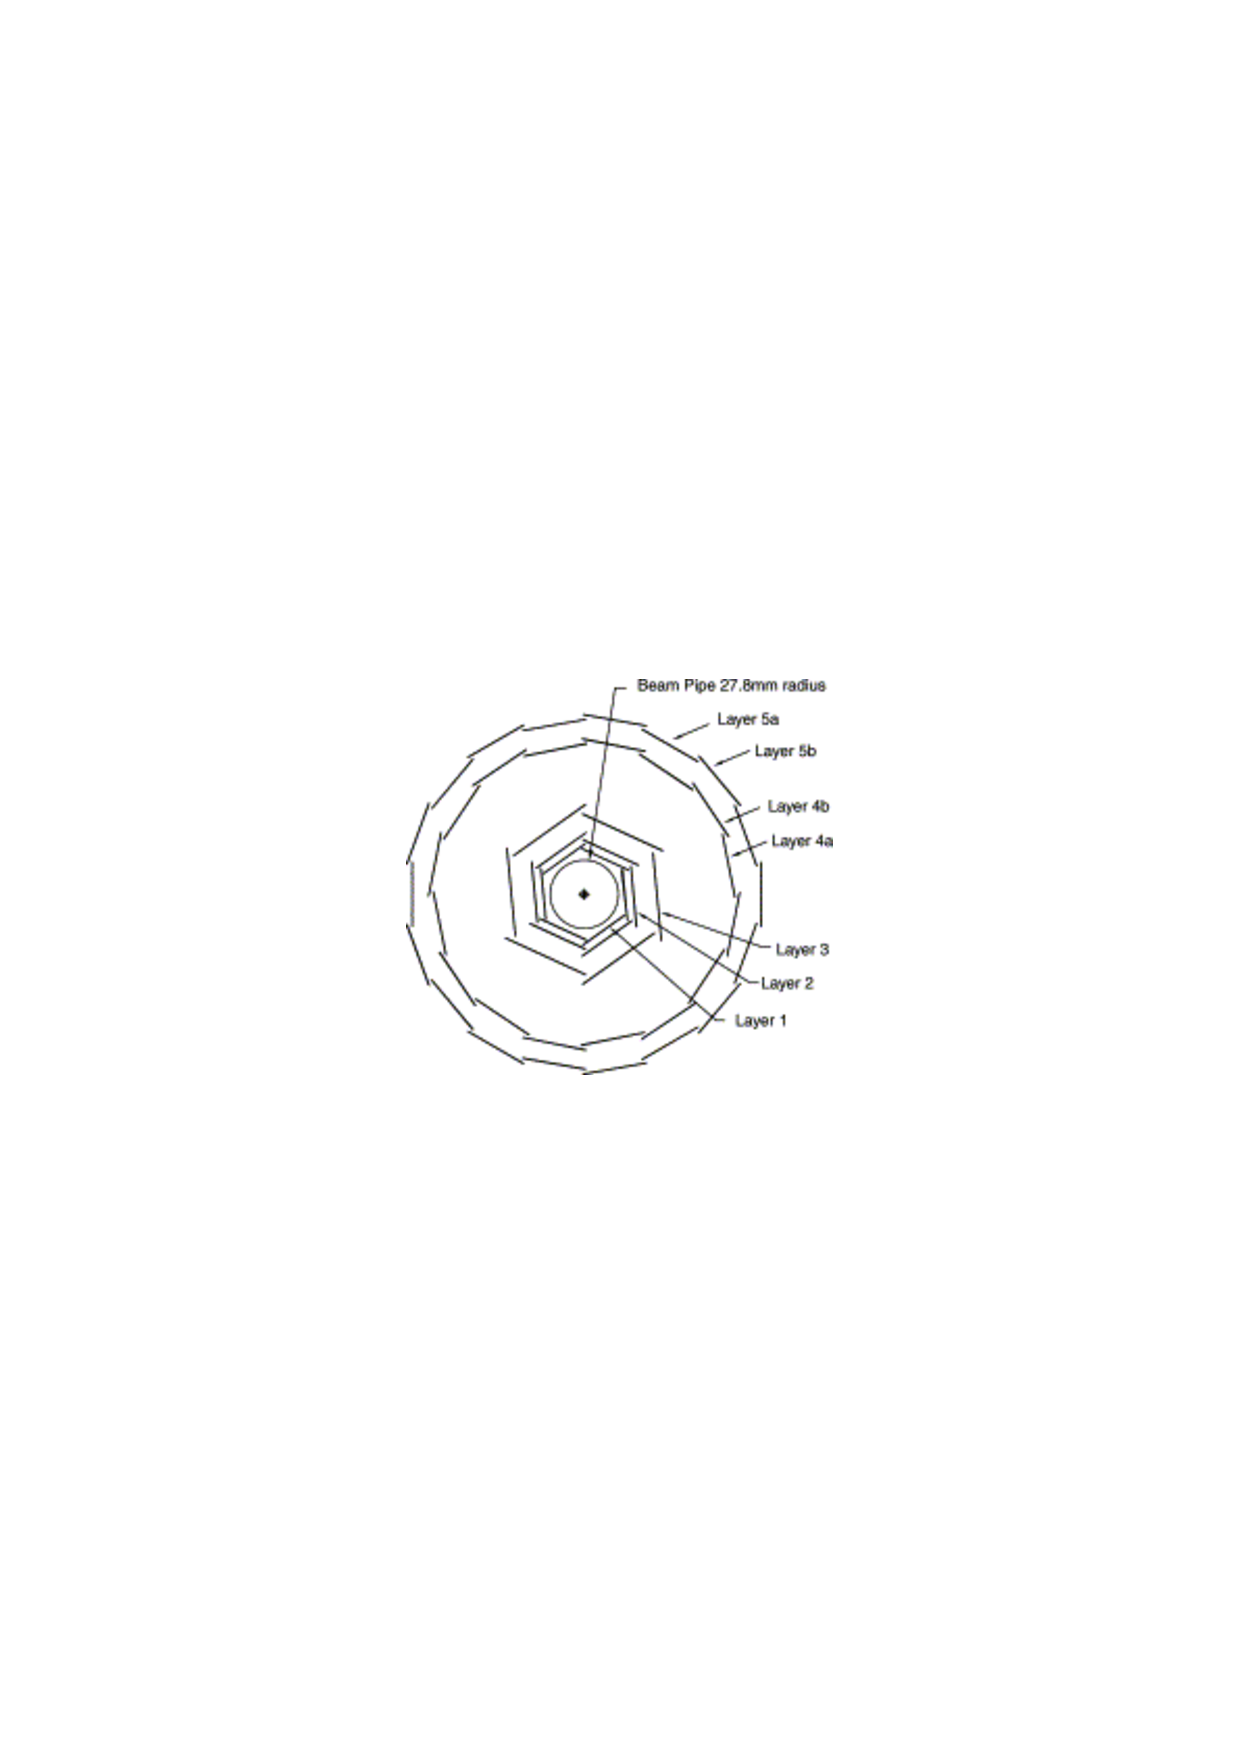
\includegraphics[width=0.45\textwidth]{miniSVT.pdf}
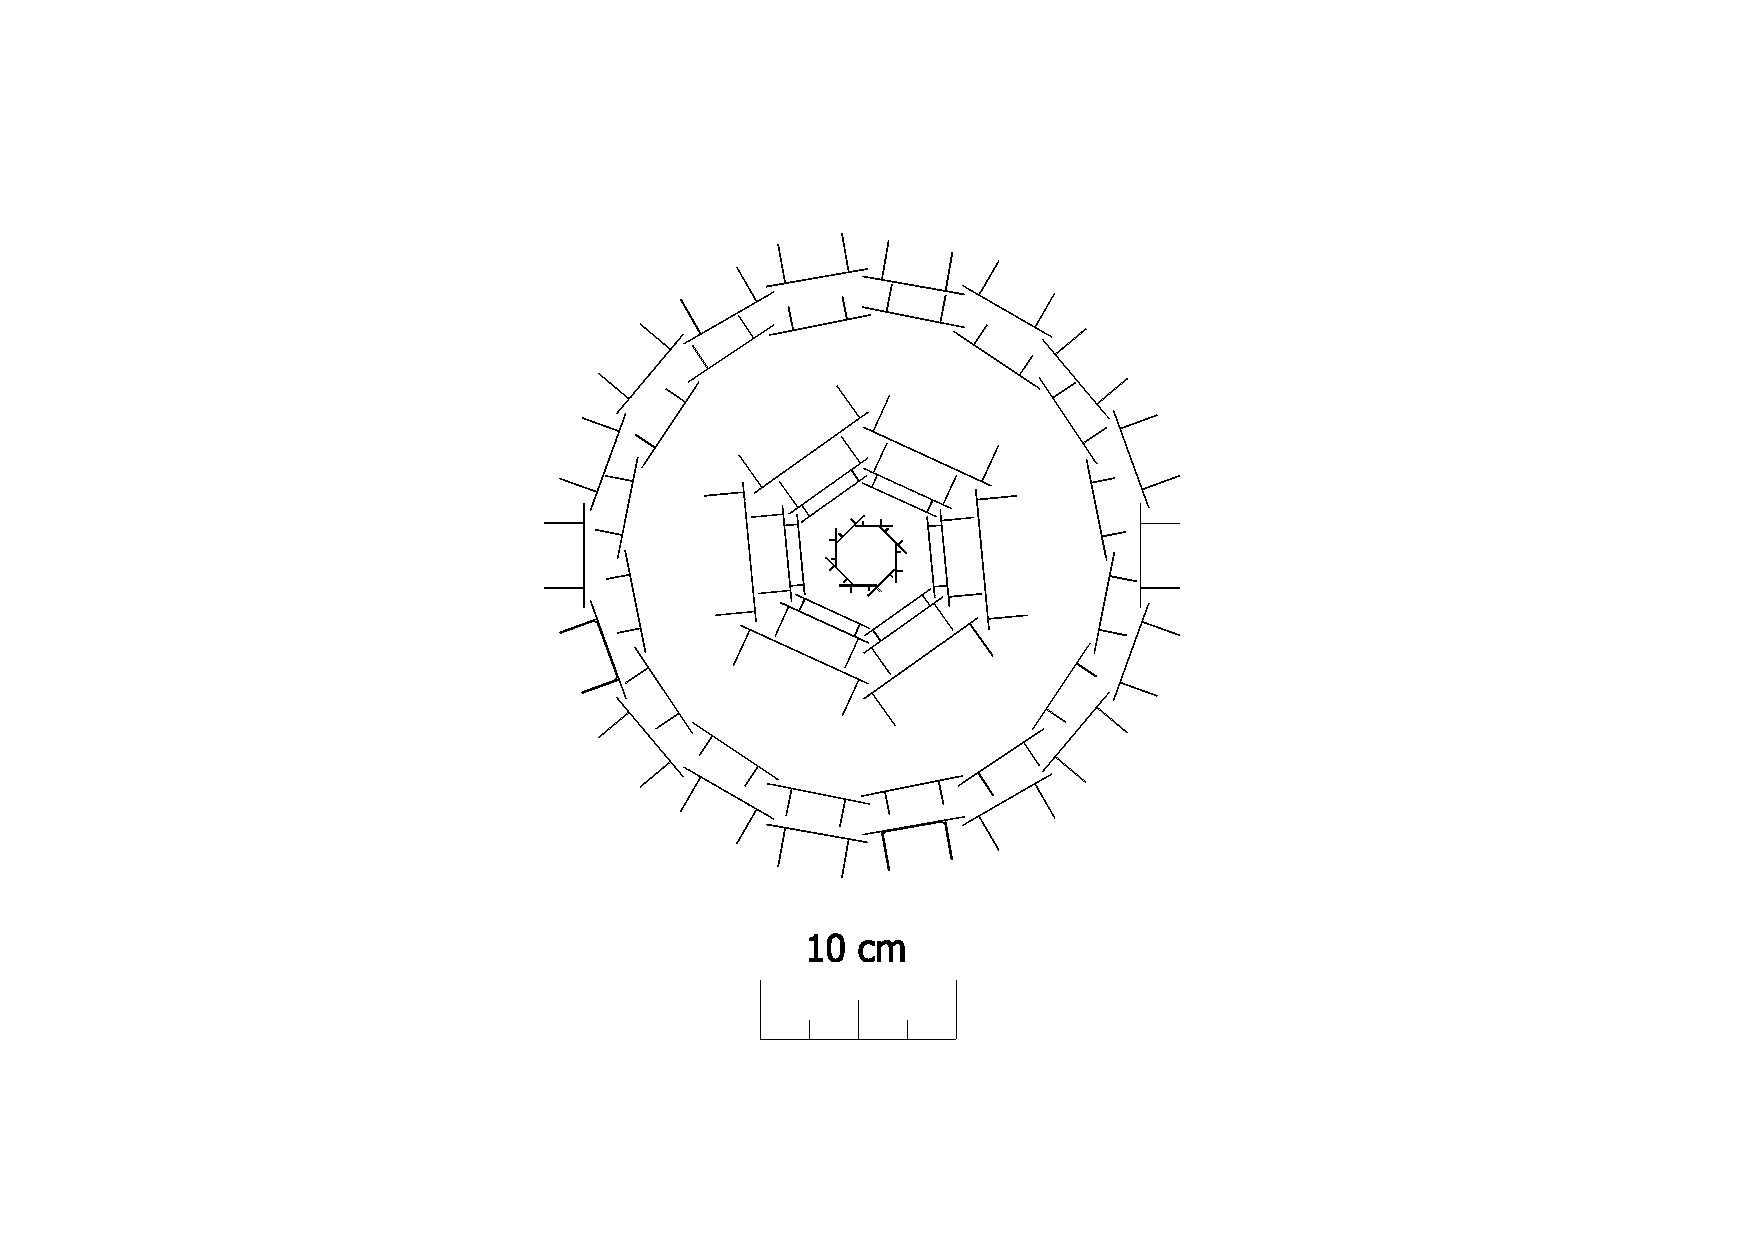
\includegraphics[width=0.45\textwidth]{miniSuperBSVT.pdf}
\caption{\label{fig:svt} (left)Schematic view of \babar\ SVT: tranverse section. (After~\cite{AUBERT20021}) The external radius is 144 mm. (right) Cross section of the SuperB SVT. (After~\cite{Baszczyk:2013xua}) }
\end{figure}


Precise vertex information, primarily extracted from precise position measurements near the 
interaction point (IP) by the SVT  is crucial to the measurement of time-dependent \CP asymmetries 
in \Bz decays, which was the  key element of the SuperB physics program. As in \babar, the SuperB 
had to be able to provide efficient and accurate tracking for  charged particles with transverse 
momenta lower than 100~MeV/c, which cannot reach the tracking Drift Chamber.

SuperB SVT had to be capable of maintaining adequate performance for time-dependent 
measurements
 in the presence of a lower boost of the center-of-mass (CM) frame
($\beta\gamma = 0.24$ compared to $\beta\gamma = 0.55$ of \babar) and much higher background,
mainly related to the increased instantaneous luminosity of about a factor of 100 larger than \babar.

The planned beam pipe featured a reduced radius of about $1.0~\cm$  which allows the positioning of 
Layer0 at
the desired average radius of about $1.5~\cm$. The additional  (with respect to \babar SVT) 
 Layer0 measurement,
along with the low radial material budget of the beam pipe ($0.42\%~X_0$)
and of Layer0 ($0.45\%~X_0$ with the striplet option - see Section~\ref{sec:Striplets}),
was crucial for improving the decay vertex reconstruction of the \B mesons and
 obtaining adequate proper-time resolution for time-dependent \CP violation measurements.

Physics simulations for the $B\to\pip\pim$ decay channel showed that to retain or improve the vertexing performance of the \babar\ SVT in the SuperB environment the following ingredients were necessary: the use of high granularity pixels (50~$\mu$m $\times$50~$\mu$m pitch), going indeed closer to the beam pipe and very low material budget~\cite{RIZZO2010585}. Results are shown in 
Figure~\ref{fig:bpipi}. 

\begin{figure}
\centering
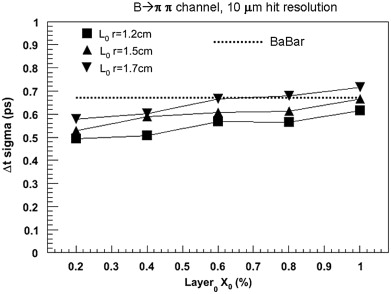
\includegraphics[width=0.45\textwidth]{bpipi}
\caption{\label{fig:bpipi} Resolution on the proper time difference of the two B mesons for the nominal SuperB boost, for different Layer0 radii, as a function of Layer0 thickness (in $X_0$ \%). The BaBar resolution for the same decay channel, is shown with a dashed line. (After~\cite{RIZZO2010585})}
\end{figure}

In summary, for the SuperB physics program a silicon tracker detector was needed with the 
capability to assure a space-point resolution of 10~$\mu$m, with a material budget below 
1\% of $X_0$, able to measure tracks with $p_T$ lower then 100~MeV/c. The real detector 
would have had to withstand a particle rate of 100~MHz/cm$^2$, mainly due to machine 
background.

\subsection{ILC}

The International Linear Collider (ILC) is a proposed $\epem$ collider. Over the years the project 
evolved and now it features a machine capable of tuning its center of mass energy in the range of 
$\sqrt{s}=250-550$~GeV, with an option for 1~TeV~\cite{ILCTDR}.  
In 2009, two detector projects (ILD \& SiD) provided a Letter Of Intent (LOI)~\cite{ILDLOI,SIDLOI}.

The ILC physics goals cover a wide and ambitious program including top quark physics, electroweak 
precision measurements, direct and indirect searches beyond the Standard Model (BSM) like SUSY, 
dark matter searches, exotic searches, etc., and a complete and extensive Higgs physics program 
covering mass, couplings to fermions and bosons, quantum numbers and total width 
measurements.  The expected level of precision for the majority of them will 
reach the percent level and will allow probing physics BSM~\cite{ILCVertexing2016}.

To accomplish this ambitious physics program stringent requirements are imposed on tracking and 
vertexing performances; these requirements didn't change much over a 
decade~\cite{ILCVertexing2007,ILCVertexing2016}. 
The  figure of merit of the future ILC vertex detector  is the impact parameter (ip) resolution which is 
expected to be:

\begin{equation}
\sigma_{ip}=5\,\mu{\rm m}\oplus\dfrac{10}{p\beta(\sin\theta)^{3/2}}\,\,\mu{\rm m\, GeV/c}
\label{eq:ILCipres}
\end{equation}

This condition demands then for: a space-point resolution of about 3~$\mu$m (hence a pitch of less 
than 20~$\mu$m; a material budget per layer of about 0.1\% of $X_0$; capabilities of performant    
tracking	down to $p_T$ of 100~MeV/c and even less.

The vertexing systems proposed by the two concept groups are both built around a central 
part based on pixel detectors; a comparison of ILD and SiD proposed solutions is presented in 
Figure~\ref{fig:ILC_concepts}. SiD features 5 pixel barrel layers and a total of 7 pixel disk layers 
per side; ILD plans for 3 double sided ladders plus , a system of pixels and strips disks  in the forward 
region.

\begin{figure}
\centering
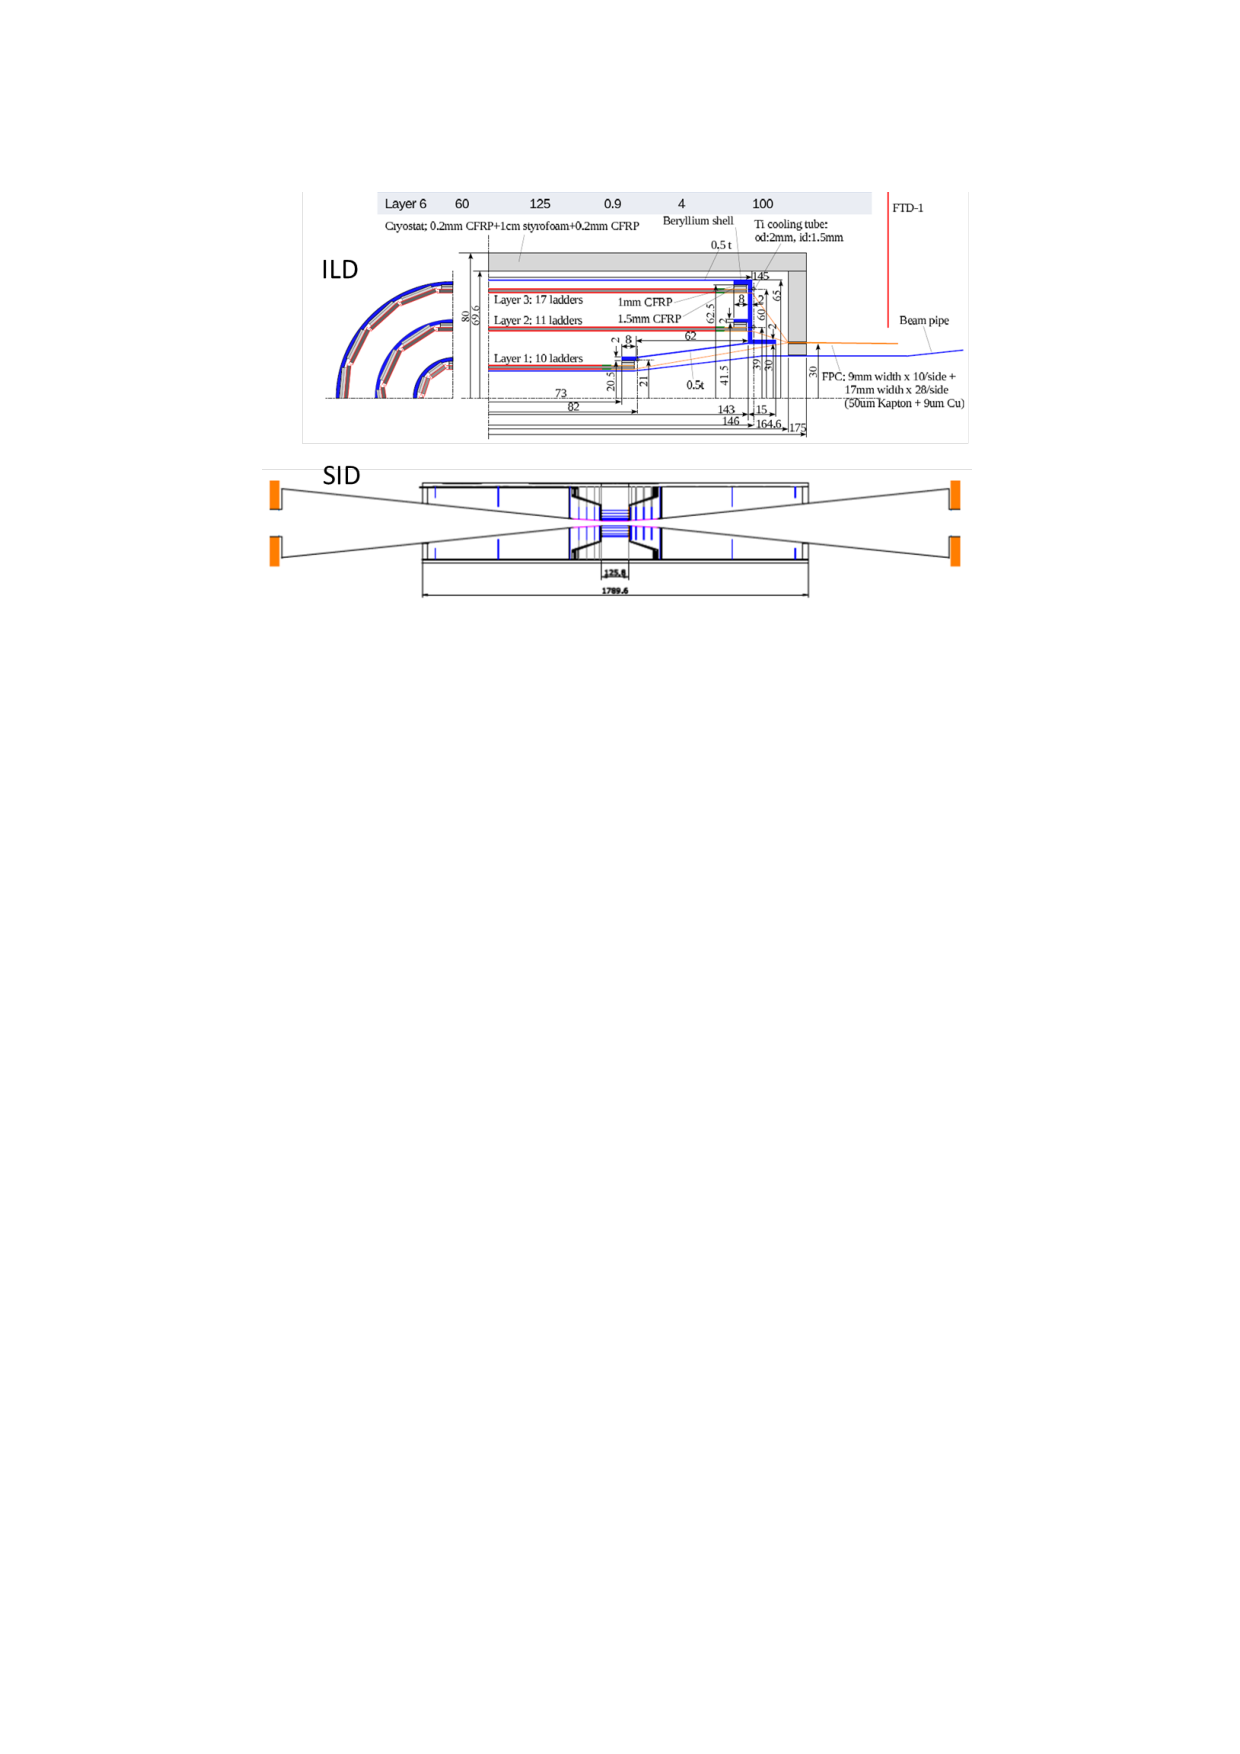
\includegraphics[width=0.5\textwidth]{ILC_concepts.pdf}
\caption{\label{fig:ILC_concepts}ILD and SiD schemes of the vertex detector (After~\cite{ILCVertexing2016})}
\end{figure}

For both vertexing detectors pixels with integrated readout (at least partial) are promising solutions, 
like CMOS MAPS, DEPFET, etc. They will assure the needed small pitch and the low material 
budget (example:~\cite{mimosa26}). 

In Summary, for the experiment at the future ILC a vertex detector with a space point resolution of 
3~$\mu$m, a material budget per layer of about 0.1\% of $X_0$ and the possibility  of    
tracking down to $p_T$ of 100~MeV/c and even less is needed.



\section{The CMOS MAPS Apsel4D}
\label{sec:Apsel4D}

As said in the introduction to this Chapter, within the SLIM5 project both pixel and strip detector
prototypes were developed. We now review the salient features of the pixel 
detector prototype, the Apsel4D. More details can be found in~\cite{BETTARINI2010942,NERI2010195}.

The Apsel4D (active pixel sensor electronics) chip was a 4096 element prototype CMOS MAPS 
detector with 
data-driven readout architecture, implementing twofold sparsification at the pixel level and at the chip. 
CMOS MAPS was the preferred solution because of the thickness of the substrate, hosting both the 
sensor and the read-out electronics, can be easily thinned down to 50~$\mu$m or less. 
The final chip featured a 4096 pixels matrix, 50$\times$50 ($\mu$m)$^2$ pitch. 
  The triple well option of CMOS commercial processes (see also Figure~\ref{fig:maps}) for the collecting electrode was exploited, implementing a full signal processing chain at the pixel level with a sparsified readout architecture. 
In Figure~\ref{fig:apsel} a picture of the Apsel4D chip is presented, together with a scheme of its architecture readout.

\begin{figure}[!htpb]
\centering
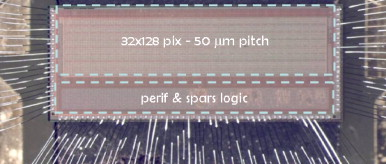
\includegraphics[width=0.45\textwidth]{Apsel.jpg}
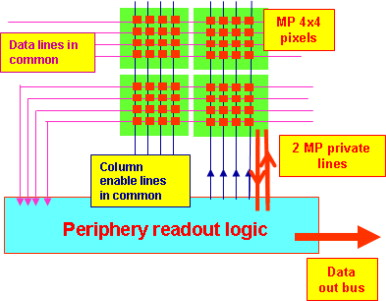
\includegraphics[width=0.45\textwidth]{Apselro.jpg}
\caption{\label{fig:apsel}(left)The Apsel4D chip bonded to the chip carrier. (right)Schematic block diagram of the architecture for MAPS matrix readout.}
\end{figure}

The elementary pixel cell includes a collecting electrode, featuring a buried deep n-type layer, and the full readout chain for signal processing~\cite{Ratti:2006zz}. The processing chain consisted of a charge 
preamplifier with charge to voltage conversion independent of the detector capacitance, a shaping 
stage featuring a 200 or 400~ns peaking time and finally a discriminator used to compare the signal witha chip-wide threshold to provide digital information. 
The design of the front-end minimized the amount of PMOS transistors and related n-wells, which act 
like competitive parasitic electrodes. The fraction of deep n-well area (electrode) over the total n-well 
area was of about 90\%. 



The readout architecture of the APSEL4D pixel, capable of performing on-chip data sparsification, was 
data-driven and permits the use of the tracker information to generate a Level 1 trigger. 
The sparsified readout was implemented thanks to the organisation of 4$\times$4 pixels into a macro 
pixel (MP); each MP had only two private lines for point-to-point connection to the peripheral logic:
one line was used to communicate that the MP has got hits, while the second private line was used to 
freeze the MP until it has been read out.  Common horizontal lines are shared among pixels in the 
same row to bring data from the pixels to the periphery, where the association with the proper 
timestamp is performed before sending the formatted data word to the output bus. The architecture is 
presented in Figure~\ref{fig:apsel}.

The chip has been designed to run with a maximum matrix readout rate of 32 hit pixels/clock cycle and 
a local buffer of maximum 160 hits to minimize the matrix sweep time.
The readout clock, designed to run up to 100~MHz, was operated at 20~MHz in the beam test.
Noise performance were estimated in the laboratory to be of about 75~e (ENC) with 20\% dispersion 
across the matrix; the threshold dispersion over the pixels was estimated be about 60~e.

\section{The Striplets Detector}
\label{sec:Striplets}

Within the SLIM5 project the DSSD detector prototype development was called ``striplets''.
The striplets detector was indeed a double-sided strip detector, realised on high-resistivity 
$n-$type bulk. A picture of the striplets detector can be seen in Figure~\ref{fig:striplets}.

\begin{figure}[!htpb]
\centering
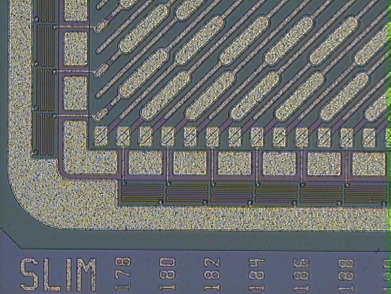
\includegraphics[width=0.5\textwidth]{striplets.jpg}
\caption{\label{fig:striplets} Detail of a corner of the SLIM5 striplet detectors.}
\end{figure}



\section{Discussion of the Performance of SLIM5 Detectors}
\label{sec:SLIM5Results}
A demonstrator was built~\cite{BETTARINI2010942}, it was composed of CMOS MAPS 
 and thin silicon DSSDs and tested it on beam at the T9 facility of the CERN PS. 


\section{Summary}
